%!TEX root = ../Dissertation.tex

\section{Functions with Costly Gradients} \label{introduction}

Optimization plays an important role in many of many branches of statistics
and machine learning. Usually, once a model has been specified, it must be
fitted. This may take the form of minimzing the loss between the model and the
data, for example, or perhaps another operational goal is desired. In either
case, this is the point where  the reigns are then handed over to an
optimization algorithm. Consider the generic unconstrained convex optimization
problem $f$ over the  reals:
\begin{equation} \label{generic-optimization}
  \underset{x\in \Real^n}{\mbox{minimize}} \quad f(x), 
  \qquad f: \Real^n \rightarrow \Real.
\end{equation}
where $f$ convex and lower semicontinuous \cite[Definition~1.5]{RTRW:1998}. In
the framework of first order optimization \cite{nemirovski2005efficient}, $f$
is thought of as a black box. Our access to $f$ is is mediated through a
subgradient oracle,

\begin{defn}[$0^{th}$ and $1^{st}$ order oracle] \label{dfn:exact-subgradient-oracle}
Let $f$ be a convex function. Then $f$ is equiped with a 0th and 1st order
oracle, $\oracle$ if
$$
(f(x), g) = \oracle(x), 
	\qquad f(\bar{x}) \geq f(x)+g^T(\bar{x}-x) 
	\quad \forall \bar{x},
$$
\end{defn}

Of course, this can be succinctly stated as $g\in \partial f(x)$. We are
interested in efficient algorithms for solving Problem \ref{generic-optimization}.
∫The first, and most direct measure of efficiency is its
arithmetical complexity. This is the number of floating point operations
necessary to drive $f(x) - \inf_x f(x)$ down to a requisite tolerance on a computer. The
second, informational complexity is the number of times which the oracle is
called to drive the accuracy of the problem down a similar amount.

To understand the distinctions between these two measures of efficiency, we
note that many optimization algorithms involves a trade-off between two
different forms  of complexity. Often, we begin with a simple model of $f$.
Next, a query to $\oracle$ is made. We then update our model of $f$
based on this new information. The model is then queried, in the form of a
subproblem, to find a new search point $x$ to query the oracle. The process
then repeats. In some extreme cases, such as the center of gravity
method\cite{levin1965algorithm}, the cost of the inner subproblem can be
exponential in the number of dimensions, but its informational complexity is
optimal. In other cases, such as sub-gradient descent, there is essentially no
work in the inner subproblems - but the algorithm requires numerous, repeated
calls to the sub-gradient. Most algorithms operate somewhere in between these
two extremes - and finding the right balance, while exploiting problem
structure, is essential to optimal performance.

In this thesis we are motivated by the modern appetite for complexity and
scale, which gives rise to functions $f$ for which a call to $\oracle$
requires a high computational load. Such functions arise, for example, when
$f$ is defined either implicitly via another optimization problem, or an
integral over a set. In either case, the cost of evaluating $\oracle$
dominates the complexity of the algorithm. Not only do we need to use gradient
information judiciously, in many cases of practical interest we do not have
the luxary of even calling $\oracle$ once, and we must resort to
approximations.

\section{Constructing Approximate Subgradient Oracles}

Approximating an oracle is an important ingredient in much of modern
optimization. As we shall soon discuss, large, expensive oracles of this
nature typically arise as a byproduct of a numerical procedures. This may be a
numerical optimizer, or a Monte-Carlo integrator. Either way, we compute our
function via an iterative procedure which can be terminated part way. As we
shall see, this partial information is usually enough to yield progress on the
optimization. We will refer to such oracles as approximate oracles. By
choosing an appropriate time to terminate this computation, this oracle
becomes controllable, giving us the liberty of trading off accuracy for
computation.

A typical algorithm which takes advantage of this proceeds as follows: in the
early parts of the optimization, we only need a rough approximation to
$\oracle$. And as we move to the stages of refinement and high
numerical accuracy, we pursue finer approximations. As we shall explore, this
scaling of the amount of work with the accuracy of the solution is typical.
And thus we can get away with nearly the same convergence rates without a
single call to $\oracle$. We will discuss the construction and examples
of approximate oracles in the next two sections.

\subsection{Parametric Minimizations/Saddle Systems} 

A first example of a function for which $\oracle$ is expensive  is one
defined implicitly as the minimization of another function. If $h(\cdot,
\cdot)$ is a convex-concave saddle function, i.e. it is convex the
first argument, and concave in the  second, then we can define $f$
as one implicitly taken after maximizing over $y$,
\begin{equation} \label{eq:saddle-f}
f(x) := \max_y \, h(x,y)
\end{equation}
We are using $\max$ instead of $\sup$ as we assume $h$ is such that 
the maximum is achieved for all $x$. Then we can construct a $0^{th}$ and $1^{st}$ order oracle by first solving the inner subproblem, to yield optimal solution $y^*$, and then differentiate with respect to $x$. In other words
\begin{equation}
(h(x,y^{*}),g)
    =\oracle(x)
      \qquad g \in \partial h(\cdot ,y^{*})(x)
      \qquad y^{*}\in\underset{y}{\mbox{argmax }}h(x,y).
\end{equation}
This is true as by the definition of the subgradient,
$$h(\bar{x},y^*) \geq h(x, y) + g^T(\bar{x} - x) = f(x) + g^T(\bar{x} - x) 
\qquad
\mbox{for any } \bar{x}, \;\; g \in \partial h(\cdot ,y^{*})(x) $$
thus matching the Definition \ref{dfn:exact-subgradient-oracle}. Such functions arise in many contexts, in particular in duality, be it
Largrangian or Fenchel (concrete examples follow shortly). 

A
second example comes from parametrized minimization. Let $f(\cdot, \cdot)$ is a
convex function. We define $f$ implicitly by minimizing over a block of variables,
\begin{equation}
f(x)=\min_{y}h(x,y)
\end{equation}
and we find ourselves in a similar situation. If we had access to the optimal solution,
then if all the level sets of $h$ are bounded (possibly empty), then by \cite{RTRW:1998} Theorem 10.13 we can differentiate under the optimization, to get a first order oracle
\begin{equation}
(h(x,y^{*}),g)
    =\oracle(x)
      \qquad g \in \partial h(\cdot ,y^{*})(x)
      \qquad y^{*}\in\underset{y}{\mbox{argmin }}h(x,y).
\end{equation}
If there is no closed form solution for the optimization, one must resort to
numerical methods. Thus, each call to the oracle requires a call to a convex
optimization program, one in principle solved to infinite floating  point
precision. This is very impractical, and as we shall see, but in both cases, it is
possible by running the optimization terminating part way, to obtain an lower 
minorant. The further $x$ is driven towards optimality, the more accurate the
oracle becomes. We will discuss three ways of measuring the accuracy of this lower
minorant. The first is the epsilon subgradient
$$
  g \in \partial_\epsilon f(x) \quad \text{and} \quad f(\bar{x}) + \epsilon \geq f(x)+{g}^T({\bar{x}-x}) \quad \forall \bar{x}
$$
which measures the distance from the lower bound at $x$ from $f(x)$, see
Figure \ref{fig:approx-oracle}. A computable version of the $\epsilon$-subgradient, 
when $f(x)$ is unknown, is

\begin{defn}[Inexact Oracle] \label{def:epi-inexact-oracle} Let $f$ be a convex
function. Then $f$ is equipped with an inexact oracle if we can find
$$(u,l,g)=\epioracle(x,\epsilon),\quad 
l+g^T(\bar{x}-x)\leq f(\bar{x}) \mbox{ for all }\bar{x}, \quad f(x) \leq u, \quad 
u-l\leq\epsilon
$$
\end{defn}

The $\epsilon$ here is computable, as we can obtain (as we shall see in the
next section) lower and upper bounds on $f$ from partial computations with an
appeal to duality. Since $l > f(x)$, $g \in \partial_\epsilon f(x)$ - this
also gives an epsilon subgradient, though a weaker one. And finally, it is
clear that $\epioracle(x,0) = \oracle(x)$. While the above are measures of
vertical distance from $f(x)$, we can also measure the error horizontally, see
Figure ~\ref{fig:approx-oracle}. This gives rise to the shallow cut oracle,
popular in the Ellipsoid method \cite{bland1981ellipsoid} literature, which
measures  the horizontal distance of the lower bound where it intersects the
horizontal line at $f(x)$ from $x$:

\begin{defn}[Shallow-cut subgradient oracle] \label{def:shallow-cut-oracle} Let $f$ be a convex
function. Then $f$ is equipped with an shallow-cut oracle if we can find
   \begin{equation} \label{eq:SpO-Oracle}
     g = \shalloworacle (x,\epsilon ) 
     \quad \text{and}\quad  
     f(x)+g^T(\bar{x}-x)\leq f(\bar{x}) 
     + \epsilon\|g\| \quad 
     \forall \bar{x}
   \end{equation}
\end{defn}

% One may pause to ask why these problems are relevant
% when one can simply attack the problem of minimizing over $x$ and $y$ simultaniously.
% We will show, in certain examples, that sometimes the opitmization over $y$ can be done
% using an existing solver, or admits special structure. We may thus
% wish to take advantage of such technology by doing the minimization sequentially.


\begin{figure} 
\begin{centering}
\includegraphics[width=0.65\textwidth]{cutting/fig0.pdf}
\par\end{centering}
\caption{Illustration of a shallow cut with an inexact epigraphical oracle. The dotted
line is $f(x)$, the polytope defined by the black solid lines $P_k$. The black
dot is center, and the two red lines are the two cutting planes provided by the 
oracle.} \label{fig:approx-oracle}
\end{figure}

Let us look at a few concrete examples illustrating how to construct an oracle of this form.

\subsubsection{Saddle Systems} For the remainder of this subsubsection, we will return to the definition of $h(\cdot, \cdot)$ in \ref{eq:saddle-f} as a saddle function defined on $\Real^n \times \Real^m$, and $f$ as $f(x) = \sup_y\ h(x,y)$. For a fixed vector $x$, any vector $\bar{y}$ in the domain of $h(x,\cdot)$
certifies a lower bound $l:=h(\bar{x},x)$. Together with any subgradient
$g\in\partial h(\cdot,\bar{y})(x)$, this lower bound generates a global affine
minorant to $f$, i.e.,
\[
  f(x) \geq h(x, \bar{y}) \ge l + g^T(x-\bar{x}) \qquad g\in\partial h(\cdot,\bar{y})(x) \qquad
\]
An upper bound is trickier to find, and requires an appeal to duality. This
often requires knowledge of the structure of $h(x, \cdot)$. We will, for
notational clarity, hide the dependence on $x$ and make $h$ convex by letting $ h(v) := -h(x,v). $
Assume that $h$ can be written as the sum of two functions,
\begin{equation}\label{eq:seperable_form_h}
h(v) = \bar{h}(Av) + \tfrac{1}{2}\|v\|^2.
\end{equation}
Assuming strong Fenchel Duality, i.e. $A \cdot \mbox{dom}(\bar{h})$ is not empty,
a weak assumption, we have
\begin{align*}
f(x) = \sup -h(x,v) = -\inf_{v}h(v) 
 & =-\inf_{v}\{\bar{h}(Av)+\tfrac{1}{2}\|v\|^{2}\} 
 \qquad (\mbox{compute fenchel dual})\\ 
 & =\inf_{y}\{\bar{h}^*(y)+\tfrac{1}{2}\|A^{T}y\|^{2}\}
 \leq\bar{h}^*(\bar{y})+\tfrac{1}{2}\|A^{T}\bar{y}\|^{2}.
\end{align*}
Thus for any $\bar{y}$, we have an the upper bound on $f$. 
We do not simply require an upper and lower bound, however. We also require
$l-u$ be controllable. This can be achieved in the by applying a
primal dual algorithm, noting that $l-u$ is exactly the duality gap.
For example, we may apply a first order method to the dual problem
$$
\underset{y}{\mbox{minimize}}\quad \bar{h}^*(y)+\tfrac{1}{2}\|A^{T}y\|^{2}
$$
for a set number of iterations. Once we have an "acceptable" $y$, we can
recover the primal with $v=-A^{T}y$. As we get closer to the optimum, $y$
approaches the dual solution, and $v$ approaches the primal solution. The
duality gap is precisely $\epsilon$. To summarize, we compute upper and lower
bounds
\begin{align*}
u =\bar{h}^*(y)+\tfrac{1}{2}\|A^{T}y\|^{2} \qquad 
l =-\bar{h}(-AA^Ty)-\tfrac{1}{2}\|A^Ty\|^{2}
\end{align*}
which, with increasing iterations, go down to $0$.  By applying an optimal
first order method to the dual, we can get the  duality gap to decrease at a
rate of $\mathcal{O}(1/k)$ where $k$ is the  number of iterations. (TODO: I've
seen this results somewhere. Track it  down). We can, alternately, attack the
saddle point problem directly with an optimal primal-dual first order method.
\begin{align*}
f(x) = -\inf_v h(v) & = -\inf_{v}\{\bar{h}(Av)+\tfrac{1}{2}\|v\|^{2}\} \\
&=-\inf_{v}\Big\{\sup_{y}\,\{y^{T}Av-\bar{h}^{*}(y)\}+\tfrac{1}{2}\|v\|^{2}\Big\} 
 =-\sup_{y}\Big\{\inf_{v}\,\{y^{T}Av+\tfrac{1}{2}\|v\|^{2}\}-\bar{h}^{*}(y)\Big\}
\end{align*}
Any primal-dual solution $(\bar{v},\bar{y})$ will provide both an upper
and a lower bound, as shown
\begin{align*}
f(x) = -\inf_v h(v) 
&=-\sup_{y} \{-\tfrac{1}{2}\|Ay\|^{2}-\bar{h}^{*}(y) \}\leq\tfrac{1}{2}\|A\bar{y}\|^{2}+\bar{h}^{*}(\bar{y})\\
f(x) = -\inf_v h(v) &=-\inf_{v} \{\bar{h}(Av)+\tfrac{1}{2}\|v\|^{2} \} \geq -\bar{h}(A\bar{v})-\tfrac{1}{2}\|\bar{v}\|^{2}
\end{align*}
Employing an optimal primal dual algorithm, the upper and the lower bounds
converge at a rate of $\mathcal{O}(1/k)$ \cite{chen2014optimal}.

\begin{example}[Support Vector Machines with Dataset Constraints] \label{ex:dataset-constraints}
The classification problem in machine learning involves predicting labels,
here $b_i \in \{-1,1\}$ from $n$ features, $a_i \in \Real^n$. We would
like to find a vector $y \in \Real^n$ which defines a linear function $a \mapsto a^Ty$ such that for all $i$
$$a_i^Ty < 0 \; \mbox{ if }\;  b_i = -1, \qquad 
a_i^Ty \geq 0 \; \mbox{ if }\; b_i = 1.$$ 
If such a seperation is possible, the data is known as "linearly seperable". This is very
rare, however, and in general we can only hope to minimize the number mislabeled points by solving
$$
\underset{y}{\mbox{minimize}}\qquad \mathbf{1}^{T}\mathbb{I}(BAy), \qquad B = \mbox{diag}(b), \,\, A = [a_1,\dots,a_m], \,\, \mathbb{I}(x)=\begin{cases}
1 & x>0\\
0 & x\leq0
\end{cases}
$$ 
This has a simple geometric interpretation - we have a hyperplane $\{ a \mid
y^Ta = 0 \}$, the "seperating hyperplane", which as the name suggests
separates the positively labeled points from the negatively labeled ones.  We
can also define a weighted version of this problem, where each datapoint is
given a weight $w_i$, which determines its importance (if all points are
equal, $w_i = 1$). The weighted version of this problem is
$$
\underset{y}{\mbox{minimize}}\qquad w^{T}\mathbb{I}(BAy)
$$ 
This problem, unfortunately, is NP-hard. We can employ, however, the convex relaxation
$\mathbb{I}(x)\leq \max\{0, 1- x\}$ and solve the relaxation instead. This objective has
the effect of penalizing a misclassified point's distance from the decision
boundary. Let $\mathbf{1}$ be the vector of all 1's. Then we arrive at the following formulation of the problem,
$$
\underset{y}{\mbox{minimize}}\qquad w^{T}\max\{0,\mathbf{1}-BAy\}+\tfrac{1}{2}\|y\|^{2}
\qquad \quad
$$ 
a weighted support vector machine. It is
rare that the goal of minimizing misclassification error is the end in
itself, however. In this example we wish to increase the expressiveness of
this by adding constraints, such as
\begin{itemize}

\item  {Coverage}: One may wish to control how often a classifier predicts the
positive (or negative) class. For example, one may want to ensure that only
10\% of customers are selected to receive a printed catalog due to budget
constraints, or perhaps to compensate for a biased training set.

\item  {Churn}: We wish for two models to disagree only on a relatively small
number of examples near the true decision boundary

\item Fairness: A practitioner may be required to guarantee fairness of a
learned classifier, in the sense that it makes positive predictions for
members of different subgroups at certain rates.  For example, one might
require that housing loans be given equally to people of different genders.
Hardt et al. [2016] identify three types of fairness: (i) demographic parity,
in which positive predictions are made at the same rate on each subgroup, (ii)
equal opportunity, in which only the true positive rates must match, and (iii)
equalized odds, in which both the true positive rates and false positive rates
must match

\item  Recall and Precision: Requirements of real-world classifiers are often
expressed in terms of precision and recall, especially when examples are
highly imbalanced between positives and negatives. In our framework, we can
handle this problem via Neyman-Pearson classification [e.g. Scott and Nowak,
2005, Davenport et al., 2010], in which one seeks to minimize the false
negative rate subject to a constraint on the false positive rate.

\end{itemize}

\noindent
A key aspect of many of the goals of Section 1 is that we can view them as
being classification  problems defined on different datasets. For example, we
might seek to maximize the accuracy on a set of labeled examples drawn in some
biased manner, require that its recall be at least 90\% on 50 small datasets
sampled in an unbiased manner from 50 different countries, desire low churn
relative to a deployed classifier on a large unbiased unlabeled dataset, and
require that 100 given egregious examples be classified correctly. For each
constraint, we have one dataset $i$, and we can therefore, we can write our
idealized objective as:
\[
\underset{y}{\mbox{minimize}}\quad (w^0)^{T}\mathbb{I}(BAy) \qquad \mbox{s.t.}\quad (w^i)^{T}\mathbb{I}(BAy) \leq u^i
\]
This problem can be relaxed using the same technique to yield the convex program
\[
 \mbox{minimize} \qquad (w^{0})^{T}\max\{0,e-L^{0}A^{0}y\}+\tfrac{1}{2}\|y\|^{2} \quad \mbox{s.t} \quad (w^{i})^{T}\max\{0,e-L^{i}A^{i}y\}\leq u^{i}
\]
We will solve this via Lagrangian Duality. The Lagrangian is
$$
\mathcal{L}(x,y)=y^{T}u+g(y)\qquad g(y)=(w^{0})^{T}\!\max\{0,e-L^{0}A^{0}y\}+{\textstyle \sum_{i=1}^{m}}y_{i}(w^{i})^{T}\!\max\{0,e-L^{i}A^{i}y\}+\tfrac{1}{2}\|y\|^{2}
$$
Observe $g$ takes the form of a weighted support vector machine, with weights
\[
g(y)\overset{\mbox{\tiny def}}{=}-\mbox{\ensuremath{\inf}}_{x}\left\{ w_{\lambda}^{T}\max\{0,\mathbf{1}-BAy\}+\tfrac{1}{2}\|y\|^{2}\right\} \quad 
w_{\lambda}^{i}=\begin{cases}
w^{0} & \mbox{if \ensuremath{i=0}}\\
\lambda_{i}w^{i} & \mbox{if \ensuremath{i\neq0}}
\end{cases},\quad 
\begin{array}{c}
L=[L^{0},\dots,L^{m}]\\
A=[A^{0},\dots,A^{m}]
\end{array}
\]
Since strong duality holds, $\sup_{y\geq0}\inf_{x}\mathcal{L}(x,y)=\inf_{x}\sup_{y\geq0}\mathcal{L}(x,y)$. Therefore each computation of $g$ requires the solution of a weighted SVM.
Using Fenchel duality, we can derive the primal dual pairs for the
problem
\begin{equation}\label{eq:svm-dual-form}
-\mbox{\ensuremath{\inf}}_{x}\left\{ w_{\lambda}^{T}\max\{0,e-BAy\}+\tfrac{1}{2}\|y\|^{2}\right\} =\inf\left\{ \mathbf{1}^{T}v-\tfrac{1}{2}\|A^{T}v\|^{2}\mid0\leq v\leq w_{\lambda}\right\} 
\end{equation}
And thus, any feasible primal dual pair will give us an upper and
lower bound. Given such a pair $(\bar{v},\bar{y})$, we can write the upper and
lower bounds as
\begin{align*}
u & =e^{T}\bar{v}-\tfrac{1}{2}\|A^{T}\bar{v}\|^{2},\qquad0\leq\bar{{v}}\leq w_{\lambda}\\
l & =w_{\lambda}^{T}\max\{0,\mathbf{1}-BA\bar{y}\}+\tfrac{1}{2}\|\bar{y}\|^{2}\\
g_{i} & =w^{iT}(\max\{0,e-B^{i}A^{i}\bar{y}\}-v^{i})
\end{align*}

\end{example}

\subsubsection{Constructing an Inexact Oracle - Parametrized Optimization} 
The parametrized optimization problem is in some sense the dual of the above problem. Here, finding an upper bound on $f$ is easy, as
\[
  f(x)=\inf_{y}h(x,y) \leq h(x,\bar{y})
\]
for any $\bar{y}$. Obtaining a lower bound, however, depends on duality. 

As in the previous section, we consider the case where our objective, as a function
of $y$ has separable structure:
\[
h(x,y) = \bar{h}(x,Ay)+\tfrac{1}{2}\|y\|^2
\]
an application of Fenchal Duality gives the following lower bound
\begin{align*}
f(x)=\inf_{y}h(x,y) & =\inf_{y}\big\{\bar{h}(x,Ay)+\tfrac{1}{2}\|y\|^{2}\big\}\\
 & =-\inf_{v}\big\{\bar{h}(x,\cdot)^{*}(v)+\tfrac{1}{2}\|A^{T}v\|^{2}\big\}\geq-\bar{h}(x,\cdot)^{*}(\bar{v})-\tfrac{1}{2}\|A^{T}\bar{v}\|^{2}.
\end{align*}
Noting that $g(x)=-\bar{h}(x,\cdot)^{*}(\bar{v})$ is a convex function, linearizing this will yield the linear lower bound we seek, with
\[
l=-h(\bar{x},\cdot)^{*}(\bar{v})-\tfrac{1}{2}\|A^{T}\bar{v}\|^{2},\qquad g\in\partial_{x}[\bar{h}(x,\cdot)^{*}(\bar{v})](\bar{x}).
\]
We are once again in a situation where our upper and lower bounds define a duality gap. Using a primal dual solver will yield a controllable inexact oracle.
% \begin{figure}
% \begin{centering}
% \includegraphics[scale=0.7]{fig0}
% \par\end{centering}
% \caption{Illustration of a shallow cut with an inexact epigraphical oracle. The dotted
% line is $f(x)$, the polytope defined by the black solid lines $P_k$. The black
% dot is center, and the two red lines are the two cutting planes provided by the 
% oracle.} \label{fig:shallow-cut}
% \end{figure}


\begin{example}[Two-Stage Stochastic Linear Programs]
In system design we are often interested in designing a system where there are multiple actors $y_i$, each acting in their own self interest based on partial information, $q_i, W_i, d_i.$ The system in which they act upon is parametrized
by $x$, and their actions have utility $Q_i(x)$.
$$
\underset{x}{\mbox{minimize}}\quad f(x) = e^{T}x+\sum_{i=1}^m Q_{i}(x),\qquad Q_{i}(x)=\inf_{y}\left\{ q_{i}^{T}x\mid W_{i}y=d_{i}-T_{i}x,y\geq0\right\} 
$$
We wish to design an optimal system, taking into account the self interested nature of the individual actors. This is a nested minimization problem - evaluating $x$ requires a solution to a linear program. By LP duality, we can get
a lower bound for each individual $Q_i$, as shown
$$
Q_{i}(x)=\inf_{y}\left\{ q_{i}^{T}x\mid W_{i}y=d_{i}-T_{i}x,y\geq0\right\} =\sup_{v}\left\{ (d_{i}-T_{i}x)^{T}v\mid W_{i}v\leq q_{i}\right\} 
$$
And thus any feasible $v$ furnishes a linear lower bound on an individual $Q_i$ and any feasible $y$ furnishes an 
upper bound. $\epsilon$ here is the duality gap. And hence by using any primal-dual linear programming solver, we can drive the error down arbitrarily.


\end{example}

\begin{example}[Bias in a Support Vector Machine] There is a large amount of research
which goes into solving the optimization problem of \eqref{ex:dataset-constraints}.
Highly optimized codes such as {\tt LIBLINEAR} \cite{REF08a} scales efficiently to hundred or thousands of
datapoints. 

The formulation of the SVM in  \eqref{ex:dataset-constraints}, has a shortcoming.
We often desire our objective to be invariant to shifts in the
decision boundary, however, i.e. a boundary of $\{ a \mid a^Tx \leq b \}$ has the same
objective for any $b$. Though this can be shoehormed in by adding a vector of $1$'s to the data, 
this parameter is still penalized in the quadratic term. A SVM which is truly agnostic
to $b$ would have the objective
$$
\underset{x\in \Real ,y}{\mbox{minimize}}\qquad h(x,y) = w^{T}\!\max\{0,\mathbf{1}-L(Ay - x\mathbf{1})\}+\frac{1}{2}\|y\|^{2}
\qquad \quad$$
This formulation of the SVM however, resists the highly efficient dual methods
of coordinate descent used in packages such as {\tt LIBLINEAR} \cite{REF08a}
due to the coupling scalar $x$. A possible approach to solve this
would be to keep $x$ fixed, and minimizing simply with respect to $y$ - an SVM
without a bias term. The bias term can then be optimized via a 1D optimization
problem. Since
$$
f(x)=\inf\left\{ w_{\lambda}^{T}\max\{0,e-BAy\}+\tfrac{1}{2}\|y\|^{2}\right\} \leq w^{T}\!\max\{0,\mathbf{1}-L(A\bar{y}-x\mathbf{1})\}+\tfrac{1}{2}\|\bar{y}\|^{2}
$$
we have the following upper and lower bounds
\begin{align*}
u & =\mathbf{1}^{T}\bar{v}-\tfrac{1}{2}\|A^{T}\bar{v}\|^{2},\qquad0\leq\bar{{v}}\leq w_{\lambda}\\
l & =w^{T}\!\max\{0,\mathbf{1}-L(A\bar{y}-x\mathbf{1})\}\\
g & =\partial(w^{T}\!\max\{0,\mathbf{1}-L(A\bar{y}-\cdot\mathbf{1})\})(x)
\end{align*}
where the upper bound comes from SVM duality, described in .

\end{example}
 

\subsection{Expectations}
Another source of costly oracles comes when $f$ is defined
implicitly via an integral or expectation. Here we will consider the smooth 
minimization problem
$$
\underset{x}{\mbox{minimize}}\quad f(x) :=\mathbf{E}\,h(x,\xi) = \int \! h(x,\xi) \,d\xi .
$$
where $\xi$ is a random variable the expectation is taken over. If $h(\cdot,
\xi)$ is convex, $f$ remains convex - and if no closed form for the integral
exists, the integral must be approximated via Monte Carlo or quadrature. We
can, as in the previous section define  a controllable oracle for functions of
this form. There are three different ways of measuring the accuracy of the problem,
and hence we have three different kinds of oracles:

\begin{defn}[Stochastic First Order Oracle] \label{defn: 0-1 Epsilon Oracle} Let $e$ be a 
random variable which depends on $x$. Then $f$ is equipped with an inexact oracle if we can find
$$
g=\mbox{{\bf stochastic}-{\bf oracle}}_f(x,\epsilon), \qquad g =\nabla f(x)+e(x).
$$
We require the $\mathbf{E}[e(x)] = 0$, and there are three variations of the
stochastic oracle.

\vspace{2mm}
\begin{tabular}{l@{\ }ll}
  A. &[Variance] &$\mathbf{E} \|e(x)\|^2 \leq \epsilon$;
  \\[6pt]
  B. &[High Probability] & $
  \Pr\left(e(x)_i \geq\delta\mid x\right)
  \leq\exp\big({-\delta^{2}/\epsilon}\big)$ \quad \mbox{for all $i$}
\\[6pt]
C. &[Deterministic] &$\|e(x)\|^2 \leq \epsilon$.
\end{tabular}
\end{defn}

These conditions are ordered in increasing strength: if (C) holds,
then (B) holds by Serfling's inequality
(Theorem~\ref{thm:Serfling Bound}), and if (B) holds, then
(A) holds because the exponential bound implies a bound on the second
moment, i.e.,
\[
\mathbf{E} \big[[e(x)_{k}]_{i}^{2}\mid \mathcal{F}_{k-1}\big] = \int_{0}^{\infty}\!\! 
\Pr([e(x)_{k}]_{i}^{2} \geq \epsilon\mid\mathcal{F}_{k-1})\,d\epsilon \leq \int_{0}^{\infty}\!\!
\exp\big({-\epsilon^{2}/U_{k}}\big)\,d\epsilon < \infty.
\]

\subsubsection{Constructing Inexact Oracles - Sampling} The basis of
quadrature and monte-carlo approaches to solving an integral all revolve
around representative evaluations of the function at well placed points. The
degree to which we can approximate this integral depends on the amount of
variation that exists within the the function. In the extreme case, if the
gradients were all equal at every point, a single sample is sufficient to
obtain the true gradient. And if the variation within the function were
tremendous, any single point would not suffice as an approximation - taken
to the extreme if the function were not integable in $\xi$. Thus our bounds
on the amount of informaiton depend on our intrustments for quantifying
the degree of variaiton of $h$ in $\xi$. There are three ways for quantifying 
this uncertainty.

\begin{hypothesis}[Uniform bounds] \label{as:pop-bounds}
  We wish to posit that for all $x,\xi$ one of the following hypothesis hold
\vspace{2mm}

\begin{tabular}{l@{\ }ll}
  A. &[Variance] & $\frac{1}{m}\sum_{i=0}^{m}\mathbf{E}\|\nabla_x h(x,\xi_{i})-\mathbf{E}[\nabla_x h(x,\xi_{i})]\|^{2}\leq B_{A}$;
  \\[6pt]
  B. &[Exponential Tail] & $\sup_{x}
  \left\{ \max_{\xi}\, [\nabla_x h(x,\xi)]_{i} -
  \min_{\xi}\,[\nabla_x h(x,\xi)]_{i}
  \right\}< B_B,
  $ \\[6pt]
  C. &[Deterministic] &$\|\nabla_x h(x,\xi)\|^2 \leq B_C$.
\end{tabular}
\end{hypothesis}

We now discuss concrete examples of this oracle.

\subsubsection{Sampling With Replacement} Since the gradient is 
a linear operator, under very weak conditions we can move the gradient
inside the expectation, $\nabla_x \mathbf{E} h(x,\xi) = \mathbf{E} \nabla_x h(x, \xi)$.
And hence if we could obtain a uniform sample from $\xi_i$, we can construct an 
estimate of the gradient sampling $m$ gradients at these instantiations:
$$
g = \oracle(x,\epsilon),\quad g = \sum_{i=0}^m \nabla_x h(x,\xi_i), \quad e(x) = \frac{1}{m} \sum_{i=0}^m \nabla_x h(x,\xi_i) - \mathbf{E} [\nabla_x h(x,\xi_i)]
$$
Our error term $e(x)$ for this estimator is sampling error, which clearly has expectation 0. 
\begin{description}

\item[(A) Variance Stochastic Oracle] The weakest of the three oracles only
requires Hypothesis \ref{as:pop-bounds}(A), a bound on the variance of the problem. Taking expectations of
$\|e(x)\|$,
\begin{align*}
\mathbf{E}\|e(x)\|^{2}=\frac{1}{m^{2}}\sum_{i=0}^{m}\mathbf{E}\|\nabla_x h(x,\xi_{i})-\mathbf{E}[\nabla_x h(x,\xi_{i})]\|^{2}\leq\frac{B_{A}}{m}
\end{align*}
Thus, to achieve an error of $\epsilon$, one needs at least $$m = \left\lceil \frac{B_A}{\epsilon} \right\rceil \quad \mbox{samples.}$$

\item[(B) High Probability Stochastic Oracle] The high probability bounds
stem from Hoeffling's inequality, applied with random variable $X_i = \nabla_x f(x,\xi_{i})_i$
$$
\Pr\left(e(x)_i \geq\delta\right)=\Pr\left(\nabla_x h(x,\xi_{i})_i-\mathbf{E}[\nabla_x h(x,\xi_{i})_i] \geq\delta\right)\leq\exp\Big(\frac{-2m\delta^{2}}{B_B^{2}}\Big)
$$
which shows that if a random variable is
bounded, its tails are not heavy. Therefore, if Hypothesis \ref{as:pop-bounds}(A) holds, then we need
$$m = \left\lceil \frac{B_B^{2}}{2\epsilon}\right\rceil \qquad \mbox{samples} $$ to get a high probability oracle. 

\item[(C) Deterministic Stochastic Oracle] We cannot construct a
controllable deterministic oracle. No matter how many samples we take, there is
a small but nonzero chance the error will not drop - for example if the same
sample repeated every time. 

\end{description}

\subsubsection{Sampling Without Replacement} We
will note an important special case. When $\xi$ takes on a finite number of
values with uniform probability, then $f$ is equivalent to the familiar case
of sums of functions
\begin{equation*} \label{eq:29}
h(x,\xi)=\frac{1}{M}\sum_{i=1}^{M}h_{i}(x),
\end{equation*}
Such sums of functions, typically with very large $M$, arise very often in
machine learning and statistics, as we shall see in the following example.


\begin{example}[Minimizing Loss] A common theme in statistics and
machine learning is the fitting of a set of observations,
$\{a_i\}_{i=1}^m \in \Real^n$ to a set of targets $\{b_i\}_{i=1}^m$. In 
linear regression, we wish to find a set of weights, $x$, for which
$x^Ta_i \approx b_i$.  To do so, we minimize over the misfit of
a model over a loss function taken over dataset. Therefore 
\begin{align*}
h_{i}(x) & =\tfrac{1}{2}(a_{i}^{T}x-b_{i})^{2}
\end{align*}
In binary classification, as discussed in Example \ref{ex:dataset-constraints} is when
$b_i$ are a set of labels, in $\{-1,1\}$. As in the case of SVMs
, we find a convex penalty to the decision boundary. Here we are interested
in loss functions which are smooth, such as
\begin{align*}
h_{i}(x) & =\log(1+\exp[-b_{i}a_{i}^{T}x]) & \mbox{Logistic Regression}\\
h_{i}(x) & =\max\{0,(b_{i}a_{i}^{T}x)^{2}\} & \mbox{Smooth SVM}
\end{align*}
These are just a small sample of possible convex loss functions defined for
pieces of data.
\end{example}

When the sum is finite, we can improve over independent sampling - we can take
samples without replacement. This reduces the number of samples we need to 
control $\epsilon$, because as we approach $M$, our population size, our error
goes to $0$.
\begin{description}
\item[(A) Variance Stochastic Oracle] If we assume  $$
\mathbf{E}\|e(x)\|^{2} = 
\left(\frac{M-m}{M}\right)\frac{\frac{1}{m}
\sum_{i=0}^{m}\mathbf{E}\|\nabla h_i(x)-\mathbf{E}[\nabla h_i(x)]\|^{2}}{m} 
\leq\left(\frac{M-m}{M}\right)\frac{B_A}{m} $$ Notice this
differs from the previous bound by a factor of $1 - m/M$. This term, known as
the finite population correction, approaches $0$ as $m$ approaches $M$, shrinking
the variance of the estimator dramatically in that regime. Therefore 
there are 
$$m= \left\lceil \frac{B_A(B_A+1)}{B_A+2M\epsilon} \right\rceil $$
samples needed to get this oracle.
\item[(B) High Probability Stochastic Oracle] The high probability bounds require
a variation of Hoeffding's inequality, Serfling's inequality which show
$$
\Pr\left(e(x)_i \geq\delta\right)=\Pr\left(\nabla_x h(x,\xi_{i})_i-\mathbf{E}[\nabla_x h(x,\xi_{i})_i] \geq\delta\right)\leq\exp\Big(\frac{-2m\delta^{2}}{B_B^{2}}\Big)
$$
Where the final step requires the assumption (C). Therefore we require
$$m=  \left\lceil \frac{B_B(B_B+1)}{B_B+2M\epsilon}  \right\rceil \qquad \mbox{samples}$$

\item[(C) Deterministic Stochastic Oracle] If we assume (C) then the
sampling error, can be bounded by
\begin{align*}
\|e(x)\|^{2} & =\Big\|\frac{M-m}{Mm}\sum_{i\in S}\nabla h_{i}(x)-\frac{1}{M}\sum\nabla h_{i}(x)\Big\|^{2}\\
 & \leq\left(\frac{M-m}{Mm}\Big\|\sum_{i\in S}\nabla h_{i}(x)\Big\|+\frac{1}{M}\Big\|\sum_{i=1}^{M}\nabla h_{i}(x_{k})\Big\|\right)^{2}\leq4\left(1-\frac{m}{M}\right)^{2}B_C
\end{align*}
Therefore we require
$$
m=\left\lceil B_C\left(1-\sqrt{\frac{\epsilon}{4}}\right)\right\rceil, \qquad \mbox{samples}
$$
to achieve a deterministic oracle
\end{description}


\section{Algorithms with Exact Oracles}

In this section we consider two broad categories of algorithms which use the
subgradient informaiton in qualitiatively different ways. The first are the
cutting plane methods, which take advantage of the fact that the first order
oracle gives a global, lower bound. This gives us clear means of localizing
the optimum, any points which can be proven to be above any upper bound on the
optimum can be safely ignored.  These methods are typically most effective in
problems with small dimensions,  but yield optimal oracle complexity.

In moderate dimensions, the above methods are no longer suitable. However,
when our objective is smooth, the subgradient on a smooth function gives a
direction of descent. Here, we treat the subgradient as a source of local
information, and move in a step along that direction.

\subsection{Cutting Plane Methods} In this subsection we will tackle the 
generic constrained optimization problem
$$
\underset{x \in \mathcal{X}}{\mbox{minimize}}\qquad f(x), \qquad \mathcal{X} \mbox{ is convex and compact}
$$
Let $\mathcal{S}^*$ be the solution set, and $x^*$ be a point in it. A literal reading of the definition of the subgradient oracle lends itself naturally to its use as a cutting plane. Since
\[
f(\bar{x}) \geq f(x) \geq \min_x f(x)
	\quad\forall \mbox{$\bar{x}$ such that ${g^T}{(\bar{x}-x)}\geq 0$}.
\]
$\oracle$ acts as a seperation oracle between $x$ and $\Soln$.
With a single call to the $\oracle$, we now know with 
certainty that the halfspace
$$\{ x \mid {g^T}{(\bar{x}-x)}\geq 0 \} \qquad \mbox{does not contain
the optimum.}$$ 
This lends itself to the following algorithm. We begin with a compact
polytope containing at least one point in $\Soln$. Then we proceed via
the iteration
\begin{align*}
  x_{k} & = \mathbf{center}(P_k), \\
  \quad g_k &= \oracle(x_k)
\\P_{k+1} & = P_k \cap \{x \mid g_k^T(x -x_k) \leq 0 \}.
\end{align*}
There are many choices for $\mathbf{center}$, but the main aim is that all
hyperplanes through it partition the set into two approximately
evenly parts. The most well understood choices for are $\mathbf{center}$ are 
the center of gravity \cite{levin1965algorithm,newman1965location},
the maximum inscribed ellipsoid \cite{tarasov1988method}, the
volumetric center \cite{vaidya1989new}, and the analytic center
\cite{ye1996complexity}.

Cutting-plane algorithms enjoy a number of attractive properties that
set them apart from other first-order methods.  Firstly, for a fixed
dimension, the center of gravity and maximum inscribed ellipsoid
variants achieve optimal oracle complexity, up to a constant factor
\cite{nemirovski1994efficient}. Secondly, on any convex function, they
achieve a universal, linear rate of convergence
\cite{nemirovski1994efficient}. This rate of convergence,
surprisingly, is oblivious to the structure of the function itself.

These advantages come at a price. Firstly, each step of the cutting
plane algorithm requires the computation of ${\bf center}$, which may
exceed the cost of the original problem. Furthermore, though the
convergence rates of cutting plane algorithms do not depend on the
conditioning of the problem, it depends strongly on the dimension of
the problem, sometimes degrading exponentially as the dimensions
increase. It is for these reasons that these algorithms are not
practical for problems of any substantial dimension.

An alternate strategy, the Ellipsoid method \cite{bland1981ellipsoid} suggests
a different to representing the localizer. Instead of storing all the previous
cuts, we maintain an  Ellipsoid which contains the optimum. At each iteration,
the search point is the center of this Ellipsoid. The cutting plane splits the
ellipsoid into two parts, and the next Ellipsoid is the largest ellipsoid
which contains this half ellipsoid.  Since simple, concise formulas exist for
updating these Ellipsoids,  this leads to inexpensive computations. And
surprisingly, this approach is sufficient to obtain linear convergence


Let us now review a few results regarding the convergence of a few prominent
cutting plane methods. To do so, we will require the following lemma, which is
a slight variation of a remark in \cite{tarasov1988method}. For our purposes
it is helpful to define a slightly more general notion of volume, a
$d$-measure. $\volmu$ is a $d$-measure if the volume increases relative to
inclusion, $P_1 \subseteq P_2 \Rightarrow \mu(P_1) \leq \mu(P_2)$, it is
homogenious with respect to scaling, i.e. $\mu(a+AP)=\det(A)\mu(P)$. Two such
measures of $\mu$ used in this paper are the volume of $\mu$ and the volume of
the maximum inscriped ellipse of $P$.

\begin{lem}\label{lem:lem-voldecrease} Let $P$ be a convex polytope containing $x^*$. Then there exists a point on the boundary of $P$, $\bar{x}$ such that
$$
f(\bar{x})-f(x^{*})\leq\left(\max_{x\in C}f(x)-\min_{x\in C}f(x)\right)\left(\frac{\mu(P)}{\mu(C)}\right)^{1/d}
$$
\end{lem}
\begin{proof}
Following \cite{tarasov1988method},  
$$\alpha^\star = \max_{a\in\lambda}\left\{ \alpha\mid\alpha\geq0,x^*+\alpha C\subseteq P\right\}.$$ 
Let $x\submax = \mbox{argmax}_{x\in C} f(x)$. Let $\bar{x}$ be the point in which the line $[x^*, x\submax ]$ intersects $P$. Then
\begin{align*}
f(\bar{x})-f(x^{*}) & \overset{(a)}{\leq}\left(f(x\submax)-f(x^{*})\right)\frac{\|\bar{x}-x^{*}\|}{\|x\submax-x^{*}\|}\\
 & \overset{(b)}{\leq}\left(f(x\submax)-f(x^{*})\right)\alpha^\star
 \overset{(c)}{\leq}\left(f(x\submax)-f(x^{*})\right)\left(\frac{\volmu(P)}{\volmu(C)}\right)^{1/n}.
\end{align*}
$(a)$ comes from the fact that $$\frac{f(y)-f(x)}{\|y-x\|}\leq\frac{f(z)-f(x)}{\|z-x\|} \qquad x \in [y,z].$$$(b)$ comes from the fact that and $x^* + \alpha C \subseteq P$, and $(c)$ comes from the fact that $\alpha^n \mbox{vol}(C) =  \mbox{vol}(\alpha C) \leq \mbox{vol}(P).$
\end{proof}

\subsection{Epigraphical cutting plane algorithms}

We note a shortcoming of the shallow-cut subgradient oracle in
practice. Because this oracle's accuracy is measured relative to the
norm of the gradient, it is not possible to know \emph{a priori} how
much computation it requires. Another shortcoming of the algorithm
described above is that it does not make use of the objective value.
Since the objective value is often computed as a side effect of the
gradient computation, discarding this information seems wasteful. The
epigraphical cutting plane method, first suggested in
\cite{bahn1994experimental} and also described in
\cite{boyd2007localization,goffin1999two,mehrotra2000volumetric} is a
remedy to this problem. 

This oracle gives us a global lower minorant for $f$, $u + g^T(\cdot - x) \leq t$ and an upper bound on the $f(x^*)$, $u$. Operating on the lifted space $(t,x)$, the epigraphs of these two linear functions form the cutting planes which separate the current iterate $(t_k, x_k)$ from the solution, $(f(x^*), x^*)$. 
\begin{align*}
(t_{k},x_{k}) & =\mbox{\textbf{center}}(P_{k})\\
(u_{k},g_{k}) & = \oracle(x_{k})\\
P_{k+1} & =P_{k}\cap\{(t,x)\mid t\leq u_{k}\}\cap\{(t,x)\mid l_{k}+g_{k}^{T}(x-x_{k})\leq t\}
\end{align*}
Unlike the cutting plane algorithm, these two half-spaces generally do not
pass through the search point $(t_k, x_k)$. It is guaranteed, however, to do
at least better, and cut off the search point. And the cuts are typically deep - they truncate more than is strictly needed, to achieve a greater volume reduction. This comes at the price, however, of lifting the problem an extra dimension.

These methods have strong connections to bundle methods. If we define
$$
u^*_k = \min{ \{ u_0, \dots, u_{k-1}\} }, \qquad 
l^*_k(x) = \max_{i < k}\{l_i + g_i^T(x-x_i)\}.
$$Then $l^*_k$ gives a lower bound on $f$ and $u_k^*$ an upper bound on $f(x^*)$. Kelly's method \cite{kelley1960cutting} produces the next iterate by minimizing $l^*_k$ directly. Bundle methods \cite{lemarechal1975extension,wolfe1975method} regularize this approach work by minimizing $l_k^*$ with a quadratic term. Many variations of these methods exist, which we will not attempt to survey here.

Observe that for all cutting plane methods, including the ellipsoid method, $\min\{f(x_1),\dots, f(x_k)\}$ is smaller than all the points in the perimeter. Therefore we can use the above theorem to effectively determine rates of convergence. The convergence rate we get is
$$
\min\{f(x_{1}),\dots,f(x_{k})\}-f(x^{*})\leq \mbox{rate}^{k/n}\cdot\left(\max_{x\in C}f(x)-\min_{x\in C}f(x)\right)
$$
For the epigraphical variants of the cutting plane algorithm, we have the following analogous lemma

\begin{lem} \label{lem:non_strongly_convex_convergencegen}
Let  $\mathcal{K}=\mbox{{\rm conv}}\{\sup_{x\in C} f(x) \times  S,(f(x^*),x^*)\}.$
Then for an epigraphical polytope $$P =\{(t,x)\mid t\leq u^*\}\cap \mbox{\normalfont epi}(l), \qquad \mbox{for some convex lower bound $l$ on $f$}
$$
Then \[
u^*-f(x^*)\leq \left(\max_{x\in C}f(x)-\min_{x\in C}f(x) \right) \left( \frac{\volmu(P)}{\volmu(\mathcal{K})} \right)^{1/(n+1)}
\]
\end{lem}

\begin{proof}
Let $\mathcal{K}_k =\mathcal{K}\cap\{(t,x)\mid t \leq u^*_k\}$. Then 
\[
  \volmu(P_k)\overset{(a)}{\geq}\volmu(\mathcal{K}_k)\overset{(b)}{=}
  \left(\frac{u^*_k-f(x^*)}{\max_{x\in C} f(x) -f(x^*)}\right)^{n+1} \!\!\!\!\!\!\!\!\!\cdot \volmu(\mathcal{K}_0)
\]
$(a)$ comes from the fact, $P_k\supseteq \mathbf{epi}(f) \cap \{(t,x) \mid t \leq u_k\} \supseteq \mathcal{K}_k$ and
$\volmu(A)\leq\volmu(B)$ when $A\subseteq B$. $(b)$ comes from the fact
that $\mathcal{K}_k$ is just $\mathcal{K}_0$ scaled about the
base, and $\volmu(\alpha A)=\alpha^{d}\volmu(A)$.
Taking powers of $1/(n+1)$ on both sides, we yield the desired result.
\end{proof}

\subsection{Proximal Methods}

\subsubsection{Smooth Functions with Composite Structure} While smooth
optimization is useful in itself, we can, with a little effort, add a  small
amount of structurally simple nonsmoothness. We will consider the minimization
of problems with additive composite structure, i.e.
\begin{equation}
  \label{eq:minimize_fpg}
  \underset{x\in {\Real}^n}{\text{minimize}} \quad f(x) + g(x)
\end{equation}
Here we consider functions $f:\Real^n\to\Real$ and
$g:\Real^n\to\Real\cup\{+\infty\}$. Here $f$ is assumed to be smooth, and $g$
is usually simple. In machine learning applications, typically, $f$ is a loss
function that penalizes incorrect predictions of a model. $f$ contains the
data, and is typically hard to compute - but is smooth. $g$ is a regularizer
that encourages desirable structure in the solution. Important examples of
nonsmooth regularizers are the 1-norm and total variation, which encourage
sparsity in either $x$ or its gradient. Let us explore a few examples of functions
with composite structure.

\begin{example}[Feature Selection] 
The feature selection problem considers the case where
only a subset of the features are informative. The rest have no
predictive value, and should be omitted to obtain the most
parsimonious model. 
\end{example}

\begin{example}[Total Variation Denoising]
\end{example}

\begin{example}[Support Vector Machines]
\end{example}

\subsubsection{Descent Algorithms for Composite Problems}
When $f$ is smooth,
our oracle gives us gradient information, which can be interpreted as decrease
if we move an tiny amount in $d$
$$
\nabla_x f(x) = \lim_{\epsilon \rightarrow 0}\max_d f(x + \epsilon d)
$$
This information is exploited in descent methods, such as gradient
descent and its accelerated versions. In these algorithms, we make a 
small step in a descent direction - and secure a small, local amount
amount of function decrease at every iteration. 
$$
x^+ = x - \alpha \nabla f(x)
$$
We can generalize slightly to problems where $g$ isn't $0$. We begin by
discussing an interpreation of a large class of descent methods popular in
first order optimization. Given a  function $f$, differentiable at $x_k$, our
guess of the solution at  iterate $k$, we can construct a quadratic model
around $k$ as such:
\begin{align*} 
f(x) & \approx f(x_{k})+\nabla f(x_{k})^{T}(x-x_{k})+\frac{1}{2}\|x-x_{k}\|_{H}^{2} =f(x_{k})+\frac{\alpha}{2}\|x-x_{k}-\frac{1}{\alpha}\nabla f(x_{k})\|_H^{2}
\end{align*}
$H$ we will assume is a invertible, quadratic model of curvature. For
different choices of $H$, we obtain

In composite optimization, we do an identical thing. Pulling $g$ 
through and completing the square, we get
\begin{align*}
f(x)+g(x) & \approx f(x_{k})+\nabla f(x_{k})^{T}(x-x_{k})+\frac{1}{2}\|x-x_{k}\|_{H}^{2}+g(x)\\
 & =f(x_{k})+\frac{\alpha}{2}\|x-x_{k}-\frac{1}{\alpha}\nabla f(x_{k})\|_H^{2}+g(x)
\end{align*}
By minimizing the approximation, we get the next iterate. Therefore
$$
x^{+}=\underset{\bar{x}}{\mbox{argmin}}\left\{ 
\frac{1}{2}\|\bar{x}-x-H^{-1}\nabla f(x)\|_{H}^{2}
+g(\bar{x})\right\} 
$$

This is one
motivation for the definition of the proximal operator. The objective
value which the quadratic optimization takes $$
\mathbf{prox}^H_{g}(z):  =\underset{x\in\Real^{n}}{\text{argmin}}\left\{
\frac{1}{2}\|z-x\|_H^{2}+g(x)\right\}, \qquad  \mathbf{env}^H_{g}(z):
=\underset{x\in\Real^{n}}{\text{min}}\left\{
\frac{1}{2}\|z-x\|_H^{2}+g(x)\right\}  $$ And the proximal gradient
iteration is 
\begin{equation}\label{eq:prox-gradient}
x^{+}=\mathbf{prox}^\alpha_g(x-\alpha^{-1}\nabla f(x))
\end{equation}
The connection to gradient descent is clear. If $g=0$, we recover
the descent iteration. Like gradient descent, under reasonable
hypotheses they are guaranteed to achieve, within $k$ iterations, a
function value that is within $\mathcal{O}(1/k)$ of the optimal value
using a constant step size, and within $\mathcal{O}(1/k^2)$ using an
accelerated variant. \cite{Tseng:2010} outlines a unified view of the
many proximal- gradient variations, including accelerated versions
such as FISTA~\cite{beck2009fast}.

For $g$'s which are structurally simple, this it leads to an
inexpensive proximal iteration. This is not limited to, but
particularly true in the case where $g$ is separable.

When gradients of $f$ are expensive to compute, incorporate into our iterations some approximation of curvature. Suppose that $H$ is a positive-definite matrix. The iteration
\begin{equation}
  \label{eq:prox-map}
  x^{+}={\bf{prox}}^H_g(x-H^{-1}\nabla f(x))
\end{equation}
is a generalization of proximal-gradient, where $x$ is most
recent estimate of the solution, and
\begin{equation}
  \label{eq:2}
  {\bf{prox}}^H_g(z):=\underset{x\in {\Real}^n}{\text{argmin}} 
  \left\{
  \tfrac{1}{2}\|z-x\|_H^{2}+g(x) \right\}
\end{equation}
is the (scaled) proximal operator of $g$. The scaled diagonal
$H=\alpha I$ is the vanilla proximal operator described
in the previous sections. For more general matrices $H$, however,
may lead to proximal operators that dominate the computation. The
choice of $H$ remains very much an art - we are trading off complexity
in the inner subproblems for less calls to the gradient of $f$. There is an entire
continuum of algorithms that vary based on the choice of $H$, as
illustrated by Table~\ref{tab:methods}.
\begin{table}
  \caption{Preconditioned proximal-gradient methods.}
  \centering
  \begin{tabular}{l|l|l}
    %\toprule
    Method & Reference & $H$\\
    %\\\midrule
    iterative soft thresholding & \cite{beck2009fast} & $\alpha I$
    \\symmetric rank 1 & \cite{NIPS2012_4523} & $\alpha I+ss^{T}$
    \\identity-minus-rank-1 & \cite{1401.4220}  &$\alpha I-ss^T$
    \\proximal L-BFGS &\cite{schmidt2009optimizing,NIPS2014_5384,Scheinberg2016} &$\Lambda+SDS^{T}$
    % \\preconditioned proximal gradient & &$\approx\nabla^2 f(x)$ is easily invertable
    \\proximal Newton &\cite{lee2014proximal,JMLR:v16:trandihn15a,Byrd2016} & $\nabla^{2}f$
    %\\\bottomrule
  \end{tabular}
  \label{tab:methods}
\end{table}

Thee table lists a set of algorithms roughly in order of the accuracy
with which $H$ approximates the Hessian---when it exists---of the
smooth function $f$. At one extreme is iterative soft thresholding
(IST), which approximates the Hessian using a constant diagonal. At
the other extreme is proximal Newton, which uses the true Hessian. The
quality of the approximation induces a tradeoff between the number of
expected proximal iterations and the computational cost of evaluating
the proximal operator at each iteration. Thus $H$ can be considered a
preconditioner for the proximal iteration. The proposals offered by
\cite{JMLR:v16:trandihn15a} and \cite{Byrd2016} are flexible in the
choice of $H$, and so those references might also be considered to
apply to other methods listed in Table~\ref{tab:methods}.


\section{Algorithms with Inexact Oracles}


\subsection{Inexact cutting plane algorithms}

The following oracle captures such cases by only requiring an approximate
subgradient, as defined by an
$\epsilon$-subgradient~\cite[p.~219]{Roc70}.

The $\epsilon$-subgradient, too, gives us a hyperplane that separates
$x$ from $x^*$. However, this hyperplane is not guaranteed to pass
through $x$ because
\[
f(\bar{x})\geq f(x) \geq f(x^*) \quad\forall \bar{x} \quad \text{such that} \quad g^T(\bar{x}-x)\geq\epsilon, \quad g \in \partial_\epsilon f(x).
\]
If we assume for the moment that $g\ne0$, then $g^T(\bar{x}-x)$
and so we observe that the hyperplane defined by the
$\epsilon$-subgradient is displaced from $x$ in the normalized
direction $g/\|g\|$ by the amount $\epsilon/\|g\|$ from $x$. The
smaller the distance $\epsilon/\|g\|$, the more the halfspace slices
off $P$. Therefore this motivates the definition of a scaled inexact
oracle wherein we control directly the distance the hyperplane lies
from $\epsilon$.

This definition bears resemblance the definition of the shallow-cut
oracle described in the classical literature on shallow-cut ellipsoid
methods \cite{bland1981ellipsoid,grotschel2012geometric}. The main
difference is the norm in which $g$ is measured. Algorithms which use
inexact cutting planes follow this pattern. We start with
$P_0 = \mathcal{C}$. Then
\begin{align*} 
  x_{k} & =\mbox{\textbf{center}}(P_{k})\\
  \quad g_{k} &= \oracle(x_{k}, \epsilon_k) \\
  P_{k+1} & = P_k \cap \{x \mid| {g_k}^T({x -x_k}) \leq \epsilon\|g\|\}.
\end{align*}
First, a center is chosen. And then, a shallow cut oracle is called
with a specific $\epsilon_k$, one typically determined by $P_k$, to
ensure a consistent rate of decrease. When $\mathbf{center}$ is the
center of gravity, for example, Bertsimas and Vempala
\cite[Theorem~3]{bertsimas2004solving} give a bound on the guaranteed
proportion of decrease in volume if the cutting plane misses the
center of gravity by a distance $\epsilon$.


\subsubsection{Inexact Bundle Methods}

\subsubsection{}

\section{Algorithms with Stochastic Oracles}

\begin{equation}\label{eq:grad-descent}
x^+ = x - \alpha g
\end{equation}

The use of stochastic oracles have its earliest beginnings in stochastic
approximation. For smooth functions, the approximate gradient is used
as a drop in replacement of the true gradient

In general, if $\lim\inf_{k} \|e_{k}\| \neq 0$, then we necessarily
require $\alpha_k\to0$ in~\eqref{eq:grad-descent} in order to ensure optimality
of limit points. \cite[Theorem~3.4]{ComWaj2005}
show that the iteration~\eqref{eq:grad-descent} converges to a solution when
$0<\inf\alpha_k<\sup\alpha_k<2/L$ and
$\sum_{k\in\mathbf{N}}\|{e_k}\|<\infty$, and also consider other kinds
of perturbations that enter into the iteration; no convergence rates
are given.  \cite{SchmidtRouxBach:2011} link
the convergence rate of the iterations (including accelerated
variants) to $\mathbf{E} \|e_{k}\|^{2}$, which measures the variance in the
error, and to error in the computation of the projection. In the case in
which $e_k=0$ has zero mean and finite variance, it is known that the
projected-gradient method converges as $\mathcal{O}(1/\sqrt k)$; see, e.g.,
\cite{Langford:2009:SOL:1577069.1577097}. Contrast these rates
to those that can be obtained when $e_k\equiv0$, and in that case the
method has a rate of $\mathcal{O}(1/k)$, and its accelerated variant has a
rate of $\mathcal{O}(1/k^2)$, which is an optimal rate; see, e.g.,
\cite{Nes07} and \cite{BeT08}.

For the case where $g\equiv0$ (and hence the projection operator
in~\eqref{eq:grad-descent} is simply the identity map), has been extensively
studied. It is well known that if $f$ is strongly convex,
deterministic steepest descent without error (i.e., $e_k\equiv0$) and
with a constant stepsize $\alpha_k = 1/L$ converges linearly with a
rate constant $\rho<1$ that depends on the condition number of $f$;
see \cite[section~8.6]{luenberger2008linear}. \cite{BT:2000} describe conditions for convergence of the
iteration~\eqref{eq:grad-descent} when the steplengths $\alpha_k$ satisfy the
conditions $\sum_{k\in\mathbf{N}} \alpha_k = \infty$ and
$\sum_{k\in\mathbf{N}} \alpha_k^2 < \infty$. \cite{NedBer:2000} show that randomized incremental-gradient
methods for~\eqref{eq:29}, with constant steplength
$\alpha_k\equiv\alpha$, converge as 
\[ \mathbf{E}\pi_k \le \mathcal{O}(1)(\rho^k +
\alpha) \] 
where $\mathcal{O}(1)$ is a positive constant. This expression is
telling  because the first term on the right-hand side decreases at a
linear rate, and depends on the condition number through $\rho$; this
term is also present for any deterministic first-order method with
constant stepsize. For a constant stepsize, \cite{friedlander2012hybrid} give non-asymptotic rates that directly
depend on the rate at which the error goes to zero, and for the case
where $f$ is given by~\eqref{eq:29}, they further show the dependence
of the convergence rate on the sample size.


For a non-vanishing stepsize, i.e., $\liminf_{k}\alpha_k>0$,
\cite{luo1993error} show that for a decreasing error sequence that satisfies
$\|e_{k}\| = \mathcal{O} ( \|x_{k+1}-x_{k}\|)$, the function values converge to the
optimal value at an asymptotic linear rate.

The convergence in probability of the stochastic-approximation method
was first discussed by the classic 
\cite{robbins1951stochastic} paper. \cite{BT:2000} give mild conditions on $e_{k}$ and $f$
under which $f(x_{k}) \to \inf f(x)$ in probability. More recently,
\cite{nemirovski2009robust}
show that for decreasing steplengths $\alpha_k = \mathcal{O}(1/k)$, these
methods achieve a sublinear rate according to $\mathbf{E}\pi_k =
\mathcal{O}(1/k)$; the iteration average has similar convergence
properties, and it converges sublinearly with overwhelming
probability. A similar effort by \cite{nesterov2008confidence}
give exponential tail bounds for sequences with any steplength
sequence.


\section{Thesis Outline}